\chapter{Deep Learning}

\section{Was ist Deep Learning?}

Unter \textbf{Deep Learning} (zu deutsch tiefes Lernen) versteht man ein Teilgebiet des maschinellen Lernens, welches sich mit künstlichen neuronalen Netzen und große Datenmengen befasst. Es eignet sich für eine Vielzahl von Anwendungsfällen wie beispielsweiße für selbstfahrende Autos, in der Medizin als auch im Marketing. \cite{datasolut2}\\

Mit Deep Learning können Probleme gelöst werden, die ohne diese Ansätze nicht lösbar wären. Tiefes Lernen ist allerdings sehr rechenaufwändig, wodurch das Training über Monate hinweg andauern kann, um gute Entscheidungen treffen zu können. Gründe hierfür sind komplexe Architekturen sowie eine Vielzahl an Modell-Parametern. \cite{datasolut2} \\

\begin{figure}[H]
	\centering
	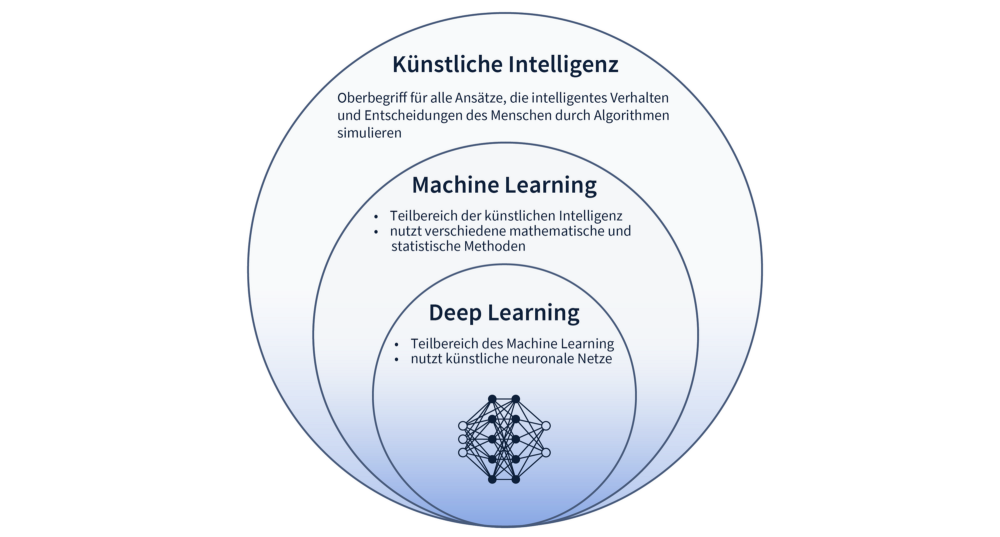
\includegraphics[width=\textwidth]{kapitel3/images/KI_Uebersicht.png}
	\label{fig:ki-übersicht}
	\caption{Übersicht Künstliche Intelligenz}
	\vspace{0.2cm}
	\quelle\url{https://datasolut.com/wp-content/uploads/2019/11/KI-und-Deep-Learning.002-e1558385989498.jpeg}
\end{figure}

Die Grundlage des Deep Learnings stellt die Verwendung von künstlichen neuronalen Netzen dar. Unter künstlichen neuronalen Netzen versteht man Algorithmen, die nach dem biologischen Vorbild des menschlichen Gehirns modelliert sind. Diese werden eingesetzt, um beispielsweise Muster in Bildern zu erkennen oder Bilder zu klassifizieren. \cite{datasolut2}\\

Ein einfaches künstliches neuronales Netz besteht dabei aus einer \textbf{Eingabeschicht} (Input Layer), einer \textbf{Zwischenschicht} (Hidden Layer) und einer \textbf{Ausgabeschicht} (Output Layer). \cite{datasolut2}

\begin{figure}[H]
	\centering
	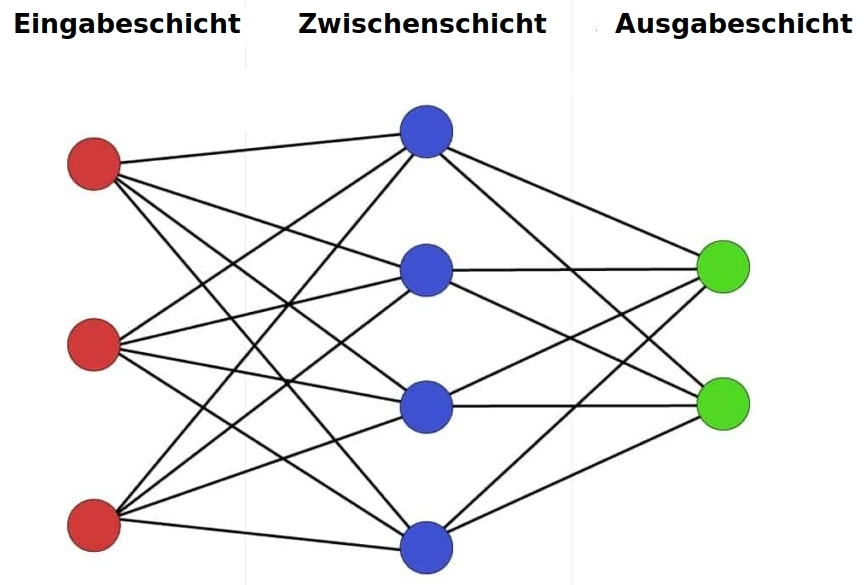
\includegraphics[width=0.65\textwidth]{kapitel3/images/Simples_Neuronales_Netz.jpg}
	\caption{Darstellung eines beispielhaften künstlichen neuronalen Netzes \\ (vereinfacht)}
	\label{fig:simples-neuronales-netz}
	\vspace{0.2cm}
	\quelle\url{https://datasolut.com/wp-content/uploads/2019/10/ku%CC%88nstliche-neuronale-Netze.jpg}
\end{figure}

Von tiefem Lernen spricht man dann, wenn die eingesetzen neuronalen Netzte mehr als eine Zwischenschicht haben.  \cite{datasolut2} 

\section{Warum Deep Learning?}

Es gibt Problemstellungen (wie beispielsweise die unstrukturierte Bilderkennung), die sich besonders gut mit künstlichen neuronalen Netzen lösen lassen. Das Erlernen dieser komplexen Muster ist jedoch mit klassischen Machine Leraning Algorithmen nur sehr schwer lösbar. Hier kommen dann tiefe künstliche neuronale Netze zum Einsatz. Je größer die Datenmenge ist, die zum lernen verwendet wird, desto besser funktioniert das tiefe Lernen. \cite{datasolut2}

\begin{figure}[H]
	\centering
	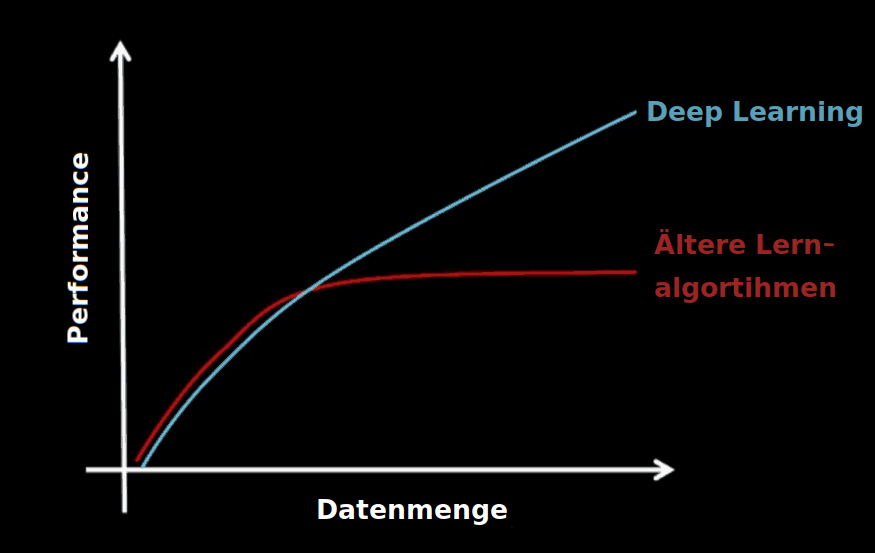
\includegraphics[width=0.65\textwidth]{kapitel3/images/Deep_Learning_Performance.png}
	\label{fig:deep-learning-performance}
	\caption{Darstellung der Performance von Deep Learning Algorithmen im Vergleich zu älteren Lernalgorithmen}
	\vspace{0.2cm}
	\quelle\url{https://datasolut.com/wp-content/uploads/2019/11/Warum-deep-learning-1024x742.png}
\end{figure}

\section{Problemstellung}

Gegeben sei ein Kamerabild $I_D$, welches von einem Duckiebot $D$ aufgenommen wurde. Das Bild $I_D$ wird einem Posenschätzer $E$ zur Verfügung gestellt, welcher dann den Abstand $d_D$ sowie die Orientierung $\Theta_D$ des Duckiebots zur rechten 
Fahrbahnmarkierung ermitteln soll. Der Posenschätzer ist hierbei ein tiefes künstliches neuronales Netz, welches die oben genannte Problemstellung lösen soll. Als Lernverfahren wird überwachtes Lernen eingesetzt.

\section{Lernverfahren}

Beim maschinellen Lernen bzw. beim Deep Learning stehen drei unterschiedliche Lernverfahren zur Verfügung:

\begin{enumerate}
	\item \textbf{Überwachtes Lernen (Supervised Learning) :}
	
	Das \textbf{überwachte Lernen} nutzt für den Lernprozess \textbf{bekannte Daten}, um daraus Muster und Zusammenhänge zu erkennen. Die Muster werden  anhand eines \textbf{Trainingsdatensatzes} (Beispieldaten) erlernt. Dabei wird der Zusammenhang zu einer Zielvariable erlernt und es wird versucht diese richtig vorherzusagen. \cite{datasolut3}
	
	\item \textbf{Unüberwachtes Lernen (Unsupervised Learning):}
	
	Das \textbf{unüberwachte Lernen} nutzt für den Lernprozess keine Beispieldaten, sondern \textbf{Rohdaten}, aus denen eigenständig Muster erkannt werden sollen. \\
	Der hauptsächliche Unterschied zum überwachten Lernen ist also, dass das unüberwachte Lernen nicht dafür ausgelegt ist, eine Vorhersage für eine bekannte Zielvariable zu treffen. \cite{datasolut3}
	
	\item \textbf{Bestärkendes Lernen (Reinforcment Learning):}
	
	Anders als das überwachte bzw. unüberwachte Lernen nutzt das \textbf{besträkende Lernen} zunächst \textbf{keine Daten}, sondern diese enstehen in einer Simulationsumgebung nach einem \textbf{Versuch-und-Irrtum-Verfahren}. \cite{der-onliner_blogspot}
\end{enumerate} 

\begin{figure}[H]
	\centering
	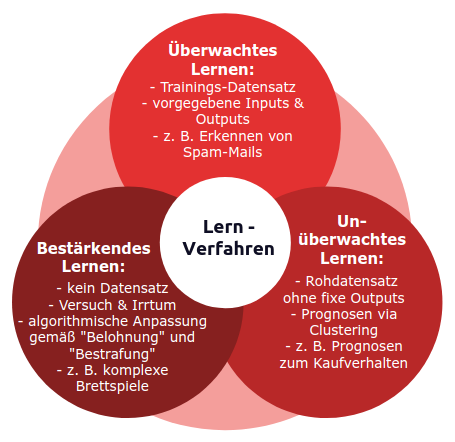
\includegraphics[width=0.6\textwidth]{kapitel3/images/lernverfahren.png}
	\label{fig:machine-learning-algorithms}
	\caption{Darstellung der verschiedenen Lernverfahren}
	\vspace{0.2cm}
	\quelle\url{https://1.bp.blogspot.com/-xstYqLb9OBw/XSYZUUD0WrI/AAAAAAAAML4/4sxvpGjIsDgmR7bDYyhcKdfM0TbvIIHdwCEwYBhgL/s400/machine-learning-lernverfahren.png}
\end{figure}

Welches Lernverfahren schlussendlich eingesetzt wird, hängt hierbei vom Anwendungsfall ab sowie mit den daraus resultierenden Datensätzen.

\section{Datensatz}

Damit der Posenschätzer seine Aufgabe erfüllen kann, muss zunächst ein \textbf{Datensatz} erstellt werden, damit dieser trainiert werden kann. Der Datensatz besteht dabei aus einem \textbf{Trainingsdatensatz}, einem \textbf{Validierungsdatensatz} sowie aus einem \textbf{Testdatensatz}. \\

Der \textbf{Trainingsdatensatz} ist ein Beispieldatensatz der für das \textbf{Lernen} der Muster und Zusammenhänge in den Daten verwendet wird. Das Modell des neuronalen Netz nutzt also diese Daten um zu lernen. \cite{datasolut} \\

Der \textbf{Validierungsdatensatz} ist ebenso ein Beispieldatensatz, welcher für die \textbf{Abstimmung der Hyperparameter} des Modells des neuronalen Netzes verwendet wird. Dadurch wird das sognenannte \glqq Overfitting\grqq{} (Überanpassung) des Modells auf die Trainingsdaten verhindert. \cite{datasolut} \\

Der \textbf{Testdatensatz} ist ebenfalls ein Beispieldatensatz, jedoch sind die Daten von den Trainingsdaten unabhängig. Die Testdaten werden beim Training des neuronalen Netzes nicht benutzt, sondern dienen zur abschließenden \textbf{Verifikation} des Modells. Dadurch kann die Qualität des Modell erfasst werden, damit man eine Aussage über die Leistungsfähigkeit des neuronalen Netzes treffen kann. \cite{datasolut} \\

Die oben genannten Datensätze wurden mit Hilfe des DuckieTown-Simulators \textbf{automatisiert} erstellt. Ein \textbf{Eintrag} eines Datensatzes besteht hierbei aus dem \textbf{Kamerabild} $I_D$, welches mit dem dazugehörigen \textbf{Abstandswert} $d_D$ sowie \textbf{Orientierungswert} $\Theta_D$ beschriftet (\glqq gelabelt\grqq) wurde. \\

Die Abbildung \ref{fig:data_entry_example} zeigt einige beispielhafte Einträge eines Datensatzes.

\begin{figure}[H]
	\centering
	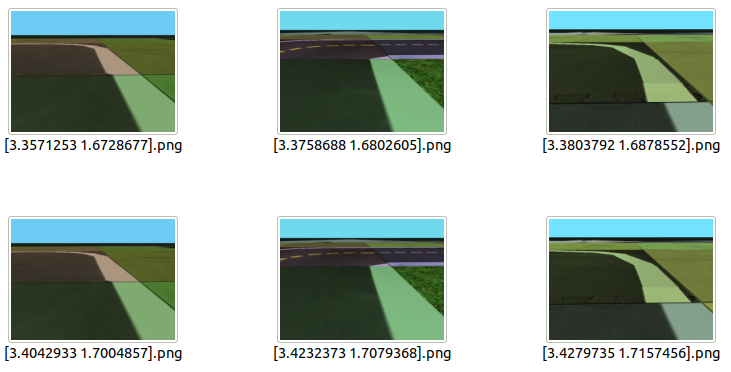
\includegraphics[width=0.8\textwidth]{kapitel3/images/dataset_entries_example.png}
	\caption{Beispielhafte Einträge eines Datensatzes}
	\label{fig:data_entry_example}
\end{figure}

\section{Funktionsweise und Aufbau künstlicher neuronaler Netze}

Die \textbf{Neuronen} (Knotenpunkte) eines künstlichen neuronalen Netzes sind \textbf{schichtweise} angeordnet. Diese werden normalerweise in einer festen Hierarchie miteinander verbunden. Die Neuronen sind dabei im Regelfall zwischen zwei Schichten verbunden, jedoch in Ausnahmefällen aber auch innerhalb einer Schicht. \cite{jaai} \\

Die Informationen fließen beginnend mit der Eingabeschicht über eine oder mehrere Zwischenschichten bis hin zur Ausgabeschicht. Dabei ist der Ausgabewert eines Neurons der Eingabewert des nächsten Neurons. \cite{jaai} \\

Künstliche neuronale Netze werden meist schematisch horizontal dargestellt (wie z.B. in Abbildung \ref{fig:simples-neuronales-netz}). Die Eingabeschicht befindet sich dabei auf der linken Seite  gefolgt von den Zwischenschichten in der Mitte und der Ausgabeschicht auf der rechten Seite.
Die Anzahl der Schichten die in einem künstlichen neuronalen Netz verwendet werden, ist eine wichtige beschreibende Information. Enthält ein Netz zum Beispiel drei Schichten, so spricht man von einem drei-schichtigen neuronalen Netz. \cite{jaai}

\subsection{Eingabeschicht}
	
	Die Eingabeschicht definiert den Startpunkt des Informationsflusses in einem künstlichen neuronalen Netz. Die Eingangssignale werden dabei von den Neuronen am Anfang dieser Schicht entgegengenommen und am Ende gewichtet an die Neuronen der ersten Zwischenschicht weitergegeben. \cite{jaai}
	
\subsection{Zwischenschichten}

	Zwischen der Eingabe- und der Ausgabeschicht befindet sich mindestens eine Zwischenschicht. Je mehr Zwischenschichten ein künstliches neuronales Netz besitzt, desto tiefer ist das Netz, jedoch bewirkt jede weitere hinzukommende Zwischenschicht auch einen Anstieg der benötigten Rechenleistung. \cite{jaai}
	
\subsection{Ausgabeschicht}

	Die Ausgabeschicht bildet die letzte Schicht eines künstlichen neuronalen Netzes, wobei diese sich hinter den Zwischenschichten befindet. Sie stellt das Ende des Informationsflusses eines künstlichen neuronalen Netz dar und enthält das Ergebnis der Informationsverarbeitung. \cite{jaai}
	
\subsection{Gewichte und Verzerrung (Bias)}


	Durch die \textbf{Gewichte} wird die \textbf{Intensität} des Informationsflusses entlang einer Verbindung eines künstlichen neuronalen Netzes beschrieben. Dazu vergibt jedes Neuron ein Gewicht für die durchfließende Information. Diese wird anschließend mit diesem Gewicht gewichtet und es wird ein Wert für die neuronen-spezifische \textbf{Verzerrung} (Bias) addiert. Das resultierende Ergebnis wird in der Regel durch eine sogenannte \textbf{Aktivierungsfunktion} geleitet, bevor es an die Neuronen der nächsten Schicht weitergegeben wird. \cite{jaai} \\
	
	Während des Trainingsprozesses werden die Gewichte und Verzerrungen so angepasst, dass das Endresultat möglichst genau den Anforderungen entspricht. \cite{jaai}
	
\subsection{Aktivierungsfunktion (activation function)}

	Aktivierungsfunktionen spielen in künstlichen neuronalen Netzen eine bedeutende Rolle, da sie dabei helfen, die komplizierte und nichtlineare funktionale Beziehung zwischen den Eingangsdaten und den abhängigen Ergebnissen zu lernen und zu verstehen. Ein Eingangssignal eines Neurons wird dabei in ein Ausgangssignal konvertiert, welches anschließend als Eingabe der nächsten Schicht verwendet wird. \cite{ai-united}
	
\subsection{Direkte Propagation}

\subsection{Backpropagation}

\subsection{Verlustfunktion (loss function)}

\subsection{Hyperparameter}

\section{Arten von  künstlichen neuronalen Netzen}





